\newpage
\section{Expectation Maximization, Mixture models}
\label{sec:EM}
Expectation Maximization (EM) is a model fitting method intended to find the maximum likelihood estimates (MLE) of the model parameters. It is designed to work with models where we wish to maximize the likelihood from which some of the parameters, the so called ``hidden variables'', are marginalized out. (For examples, see section \ref{sec:Hiararchical models}.) While direct numerical optimization of the marginal likelihood is often possible, the EM algorithm can be faster.

\subsection{Definitions}
The following terminology is going to be useful for discussing EM and mixture models. In a statistical inference problem we categorize the variables into ``observations'', ``parameters'' and ``hidden variables''.
\begin{itemize}
	\item Variables with known values are called
		\begin{itemize}
			\item {\bf observations} (or data), $D = \{x_i\}_{i=1}^N$. The models are most often designed to work with any $N$ number of observations, and often assume that the different $x_i$ are independent from each other (given the model parameters).
		\end{itemize}
	\item Variables with unknown values are often separated into two categories. (This categorization is mostly for convenience and not because of any mathematical reason. After all, all unknowns are simply values which we wish to determine through statistical inference.)
		\begin{itemize}
			\item {\bf Parameters} of the model are the unknown variables whose dimension does not increase with the number of observations $N$. Symbolically, they are $\theta = \{\theta_k\}_{k=1}^K$, where $K$ is constant, independent of $N$. Each parameter tells us something about the nature of the process that generated the observations.
			\item {\bf Hidden variables} (or hidden data) are the unknown variables whose dimension increases linearly with the number of observations. Each hidden value tells us something about the immediate circumstances of the corresponding observation.
		\end{itemize}
\end{itemize}
Since the number of hidden variables $z_i$ are the same as the number of observations $x_i$, they can be placed on the same plate in the graphical representation below.
\begin{figure}[h]
\centering
	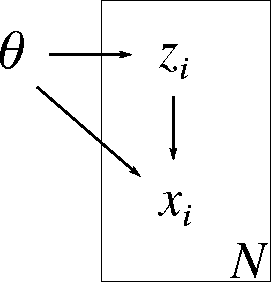
\includegraphics[height=22mm]{./figs/05-DZtheta.pdf}
\end{figure}

\subsection{Expectation Maximization}
\no {\bf The goal} of the EM methods is to find the MLE estimate in the following setting.
\begin{itemize}
	\item First, we determine the functional form of the likelihood $P(D\;|\;Z, \theta)$, and the prior on the hidden variables $P(Z\;|\;\theta)$.
	\item Second, we express the joint distribution of observed and hidden data as a product, 
	\be
		P(D, Z\;|\;\theta) = P(D\;|\;Z, \theta)\, P(Z\;|\;\theta).
	\ee
	\item Now, we wish to find the optimal $\theta$ values that maximize the marginal likelihood $P(D\;|\;\theta) = \sum_Z P(D, Z\;|\;\theta)$. This would provide a robust estimate, because, by marginalizing out $Z$, we take all possible hidden values into account.
	\be
		\theta^\text{MLE} = \amax_{\theta} \Big[\log P(D \;|\; \theta)\Big] = \amax_{\theta} \left[\log \Big(\sum_Z P(D, Z\;|\;\theta)\Big)\right]
	\ee
	\item The sum under the logarithm makes this expression difficult to analytically simplify. Although direct numerical optimization is usually feasible, EM method yields the same solution in usually fewer iterations.
\end{itemize}


\no {\bf Expectation Maximization (EM) algorithm}
\begin{enumerate}
	\item Start with realistic guess $\theta = \theta^\text{old}$
	\item E-step: Using the value of $\theta^\text{old}$, calculate the posterior distribution of $Z$: 
	\be 
		P(Z\;|\;D,\theta^\text{old}) = \frac{P(D, Z\;|\;\theta^\text{old})}{\sum_{Z'} P(D,Z'\;|\;\theta^\text{old})}
	\ee
	\item M-step: Find the optimal $\theta = \theta^\text{new}$ that maximizes the expected log likelihood, $\log P(D,Z\;|\;\theta)$, under this posterior, i.e.
	\be
		\theta^\text{new} = \amax_\theta \left[\sum_Z P(Z\;|\;D,\theta^\text{old})\log P(D,Z\;|\;\theta)\right]
	\ee
	\item Set $\theta^\text{old} \leftarrow \theta^\text{new}$, check for convergence (usually by checking if $\theta^\text{new}$ is close enough to $\theta^\text{old}$, and return to E-step if needed.
\end{enumerate}
The one-liner iteration formula, based on the likelihood $P(D,Z\;|\;\theta)$, is
	\be
		\theta^\text{new} = \amax_\theta\left[\sum_Z \frac{P(D, Z\;|\; \theta^\text{old})}{\sum_{Z'} P(D, Z'\;|\; \theta^\text{old})} \log P(D, Z\;|\; \theta)\right].
	\ee
\no Note: For each new model, the analytical formulas for the E- and M-steps need to be derived before the above algorithm can be used. The most difficult step here is simplifying two sums over $Z$, because $\sum_Z$ describes summation (or integral) over all hidden variables $\{z_i\}_{i=1}^N$,
\be
	\sum_Z [\ldots] \quad =\quad  \sum_{z_1}\sum_{z_2}\ldots \sum_{z_N} [\ldots]
\ee
In most cases it is numerically infeasible to iterate through all  value combinations of the hidden variables, the above summation needs to be simplified into a formula that prescribes summation over every data point instead.
\be
	\sum_{z_1}\sum_{z_2}\ldots \sum_{z_N} [\ldots]\qquad \rightarrow \qquad \sum_{i=1}^N[\ldots]
\ee
This is not a straightforward task.


\subsection{Mixture models}
It is common that we suspect that some data points came from one distribution while other data points from another distribution, but we do not know which came from where. Fitting a mixture model to such data can help identify the individual components and determine the origin of each data point. Let's walk through the construction of a general mixture model.
\begin{itemize}
	\item We observe data point $D=\{x_i\}_{i=1}^N$.
	\item We construct a mixture model
		\begin{itemize}
			\item with $C$ components, $c \in \{1, 2, \ldots C\}$,
			\item each of which is a distribution parametrized by $\theta_c$, so the full set of parameters is $\theta = \{\theta_c\}_{c=1}^C$.
			\item Each component is present in the mixture with a different weight $w_c \geq 0$, and the full set of weights is $w = \{w_c\}_{c=1}^C$, such that $\sum_c w_c = 1$.
		
			\item Hidden variables: The set of labels $L = \{l_i\}_{i=1}^N$, where $l_i\in \{1, 2, \ldots C\}$, indicates from which component has each data point originate.
			\item On level 1, we assume that each data point originates from the component picked out by its label, 
			\be
				P(x_i\;|\;l_i = c, \theta) = P(x_i\;|\;\theta_c).
			\ee
			\item On level 2, we describe the prior of the labels as a categorical distribution determined by the weights, 
			\be	
				P(l_i = c) = w_c.
			\ee
		\end{itemize}
		This is represented by the following graphical diagram.
	\begin{figure}[h]
	\centering
		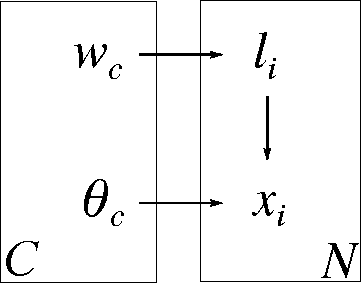
\includegraphics[height=22mm]{./figs/05-mixture.pdf}
	\end{figure}
	\item Joint distribution of data and (hidden) labels is
	\be
		P(D, L\;|\; \theta, w) = P(D\;|\;L, \theta) \;P(L\;|\;w) = \prod_{i=1}^N P(x_i\;|\;\theta_{l_i})\; w_{l_i}.
	\ee
	\item We are interested in optimizing the marginal likelihood, from which the labels are marginalized out,
	\be
		P(D\;|\; \theta, w) = \sum_L P(D, L\;|\; \theta, w) = \prod_{i=1}^N\left[\sum_{c=1}^C w_c\, P(x_i\;|\;\theta_c) \right].
	\ee

	\item The EM algorithm for this model is the following:
	\begin{enumerate}
		\item Start with realistic initial values: $\theta^\text{old}, w^\text{old}$
		\item In the E-step, calculate
		\be	
			P(l_i = c\;|\;x_i,\theta^\text{old}) = \frac{w^\text{old}_c P(x_i\;|\;\theta^\text{old}_c)}{\sum_{c'} w^\text{old}_{c'} P(x_i\;|\;\theta^\text{old}_{c'})} =: r_{i,c}
		\ee
		The value $r_{i,c}$ can be interpreted as the ``responsibility'' of component $c$ for observation $i$. For each observation, they sum to one, i.e. $\sum_c r_{i,c} = 1,\quad \forall i$.
		\item In the M-step, calculate new weights and new parameter values:
		\ba
			w_c^\text{new} &=& \frac{1}{N} \sum_{i=1}^N r_{i,c} 
			\\
			\theta_c^\text{new} &=& \amax_{\theta_c} \left[\sum_{i=1}^N r_{i,c} \log P(x_i\;|\;\theta_c)\right] 
			\\
			&=& \text{MLE of $\theta$ with data weights }\{r_{i,c}\}_{i=1}^N
		\ea
		Determining $\theta_c^\text{new}$ is not always straightforward, but even if it needs to be done numerically, it is much quicker than optimizing all components of $\theta, w$ simultaneously.
	\end{enumerate}
\end{itemize}


\newpage
\subsection{Gaussian Mixture Model}
\no Also called GMM or ``soft K-means clustering''.
\begin{itemize}
	\item We observe real-valued data points $\{x_i\}_{i=1}^N$, where $x_i \in \mathds{R}^d$, in $d$ dimensions.
	\item We construct a model that is the mixture of different multi-variate normal distributions.
	\begin{itemize}
		\item We call the components ``clusters'': $k \in \{1, 2, \ldots K\}$.
		\item Their weights are  $w = \{w_k\}_{k=1}^K$, where $w_k \geq 0$ and $\sum_k w_k = 1$.
		\item Centers of the clusters is described by the list of vectors $\mu = \{\mu_k \in \mathds{R}^d\}_{k=1}^K$
		\item Size and shape of the clusters is described by the list of covariance matrices \\ $\Sigma = \{\Sigma_k \in \mathds{R}^{d\times d}, \text{positive definite}\}_{k=1}^K$.
		\item Hidden variables are the cluster labels, $L = \{l_i\}_{i=1}^N$, where $l_i \in \{1, 2,\ldots K\}$.
		\item On level 2, we describe the prior of the labels as a categorical distribution determined by the weights,
		\ba
			P(l_i = k) &=& w_k.
		\ea
		\item On level 1, we assume that each data point comes from a multi-variate normal distribution of its cluster (picked out by its label), i.e.
		\ba
			P(x_i\;|\;l_i=k, \mu, \Sigma) &=& \text{Normal}(x_i\;|\;\mu_k, \Sigma_k) = \frac{1}{\sqrt{\det (2\pi \Sigma_k)}} \exp\left(-\frac{1}{2}(x_i - \mu_k)^\top (\Sigma_k)^{-1}(x_i - \mu_k)\right).
		\ea
	\end{itemize}
	\item The marginal likelihood, which we wish to maximize, is
	\be
		P(D\;|\;\mu, \Sigma, w) = \prod_{i=1}^N\left[\sum_{k=1}^K w_k\, \text{Normal}(x_i\;|\;\mu_k, \Sigma_k)\right].
	\ee
	\item EM algorithm
	\begin{enumerate}
		\item Choose realistic $w^\text{old}, \mu^\text{old}, \Sigma^\text{old}$ initial values. (We can choose the matrices in $\Sigma$ to be diagonal for the sake of simplicity.)
		\item In E-step, calculate the responsibilities,
		\be
			r_{i,k} = \frac{w^\text{old}_k \,\text{Normal}(x_i\;|\;\mu^\text{old}_k,\Sigma^\text{old}_k)}{\sum_{k'} w^\text{old}_{k'} \,\text{Normal}(x_i\;|\;\mu^\text{old}_{k'},\Sigma^\text{old}_{k'})}.
		\ee
		\item In M-step, calculate the new weights, and the new center and shape parameters,
		\ba
			w_k^\text{new} &=& \frac{1}{N} \sum_{i=1}^N r_{i,k} 
			\\
			\mu_k^\text{new} &=& \frac{1}{w_k^\text{new} N } \sum_{i=1}^N r_{i,k} \,x_i \\
			\Sigma_k^\text{new} &=& \frac{1}{w_k^\text{new} N } \sum_{i=1}^N r_{i,k} (x_i - \mu_k^\text{new}) (x_i - \mu_k^\text{new})^\top
		\ea
		where $(x_i)(x_i)\T$ is the outer product between two $\mathds{R}^d$ vector, which produces an $\mathds{R}^d\times \mathds{R}^d$ matrix.
	\end{enumerate}
\end{itemize}

\newpage
\no The following python class implements the EM algorithm for fitting GMM.
\begin{lstlisting}[language=python]
class GmmEm:
    def __init__(self, x):
        self.x = np.array(x)
        self.N, self.d = self.x.shape
        self.K = None
        self.weights = None
        self.means = None
        self.covs = None
    
    def initialize(self, K):
        self.K = K
        m0 = np.mean(x, axis=0)
        cov0 = np.cov(x.T)

        self.weights = [1.0/K] * K
        self.means = multivariate_normal.rvs(mean=m0, cov=cov0, size=K)
        cov_values, _ = np.linalg.eig(cov0)
        self.covs = np.array([np.eye(self.d) * 0.1 *cov_values.max()
                             for _ in range(K)])
        
    def e_step(self):
        r = []
        for k in range(K):
            r.append(self.weights[k] * 
                     multivariate_normal.pdf(self.x, 
                                             mean=self.means[k],
                                             cov=self.covs[k]))
        r = np.array(r).T
        r_sum = np.einsum('ik->i', r)
        r = np.einsum('ik,i->ik', r, 1.0/r_sum)
        return r
    
    def m_step(self, r):
        weights_new = 1.0/N * np.einsum('ik->k', r)
        means_new = 1.0/N * \
                    np.einsum('k,ik,id->kd', 
                              1.0/weights_new, 
                              r, 
                              self.x)
        deviations = np.array([self.x - means_new[k] for k in range(self.K)])
        covs_new = 1.0/N * \
                    np.einsum('k,ik,kid,kiD->kdD', 
                              1.0/weights_new, 
                              r, 
                              deviations, 
                              deviations)
        
        self.weights = weights_new
        self.means = means_new
        self.covs = covs_new
\end{lstlisting}

\newpage
\no Example: GMM in 2D with $K=2$
\begin{figure}[h]
\centering
	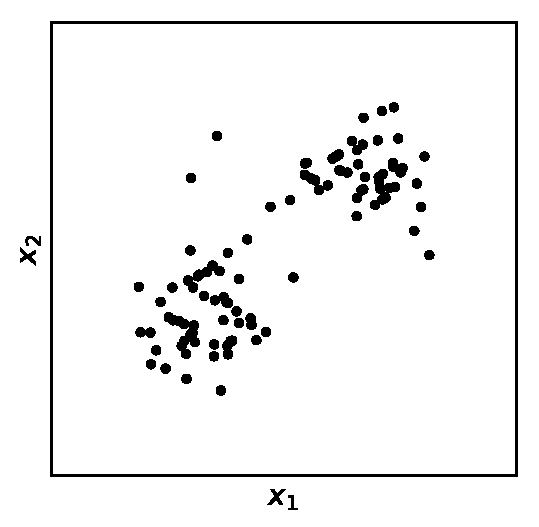
\includegraphics[width=0.30\textwidth]{./figs/05-gmm-data.pdf}
\end{figure}

\no Iterating the E- and M-steps a couple of times, we arrive to the final set of $r$ values.
\begin{lstlisting}[language=python]
gmm = GmmEm(x)

K = 2
gmm.initialize(K)
for it in range(12):
    r = gmm.e_step()
    gmm.m_step(r)
\end{lstlisting}

\begin{figure}[h!]
\centering
	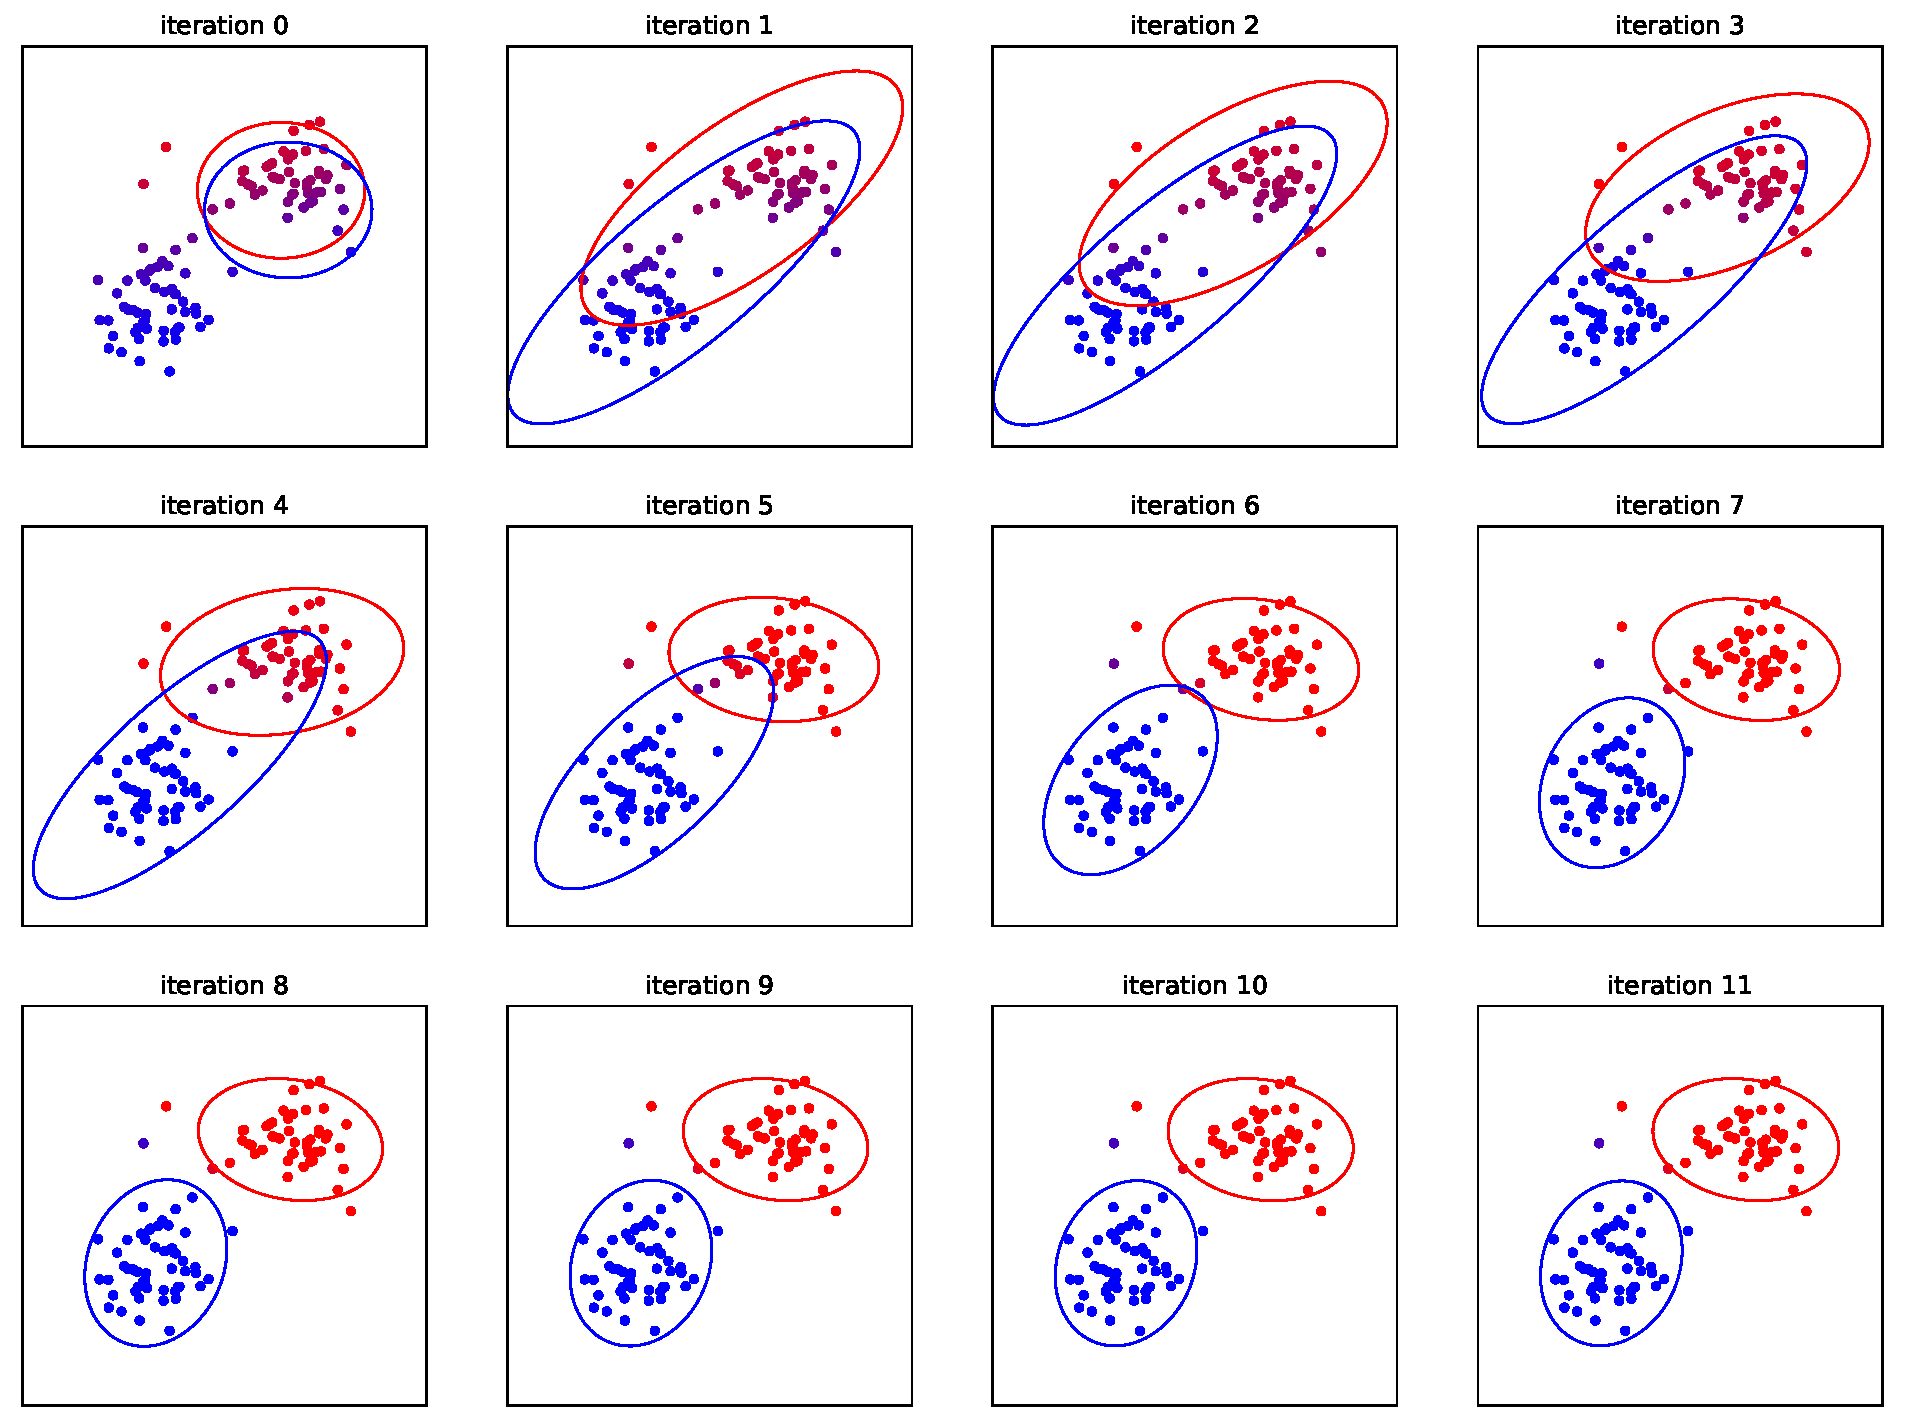
\includegraphics[width=0.93\textwidth]{./figs/05-gmm-iterations.pdf}
\end{figure}





